\subsection{后端设计}

\begin{figure}[H]
  \centering
  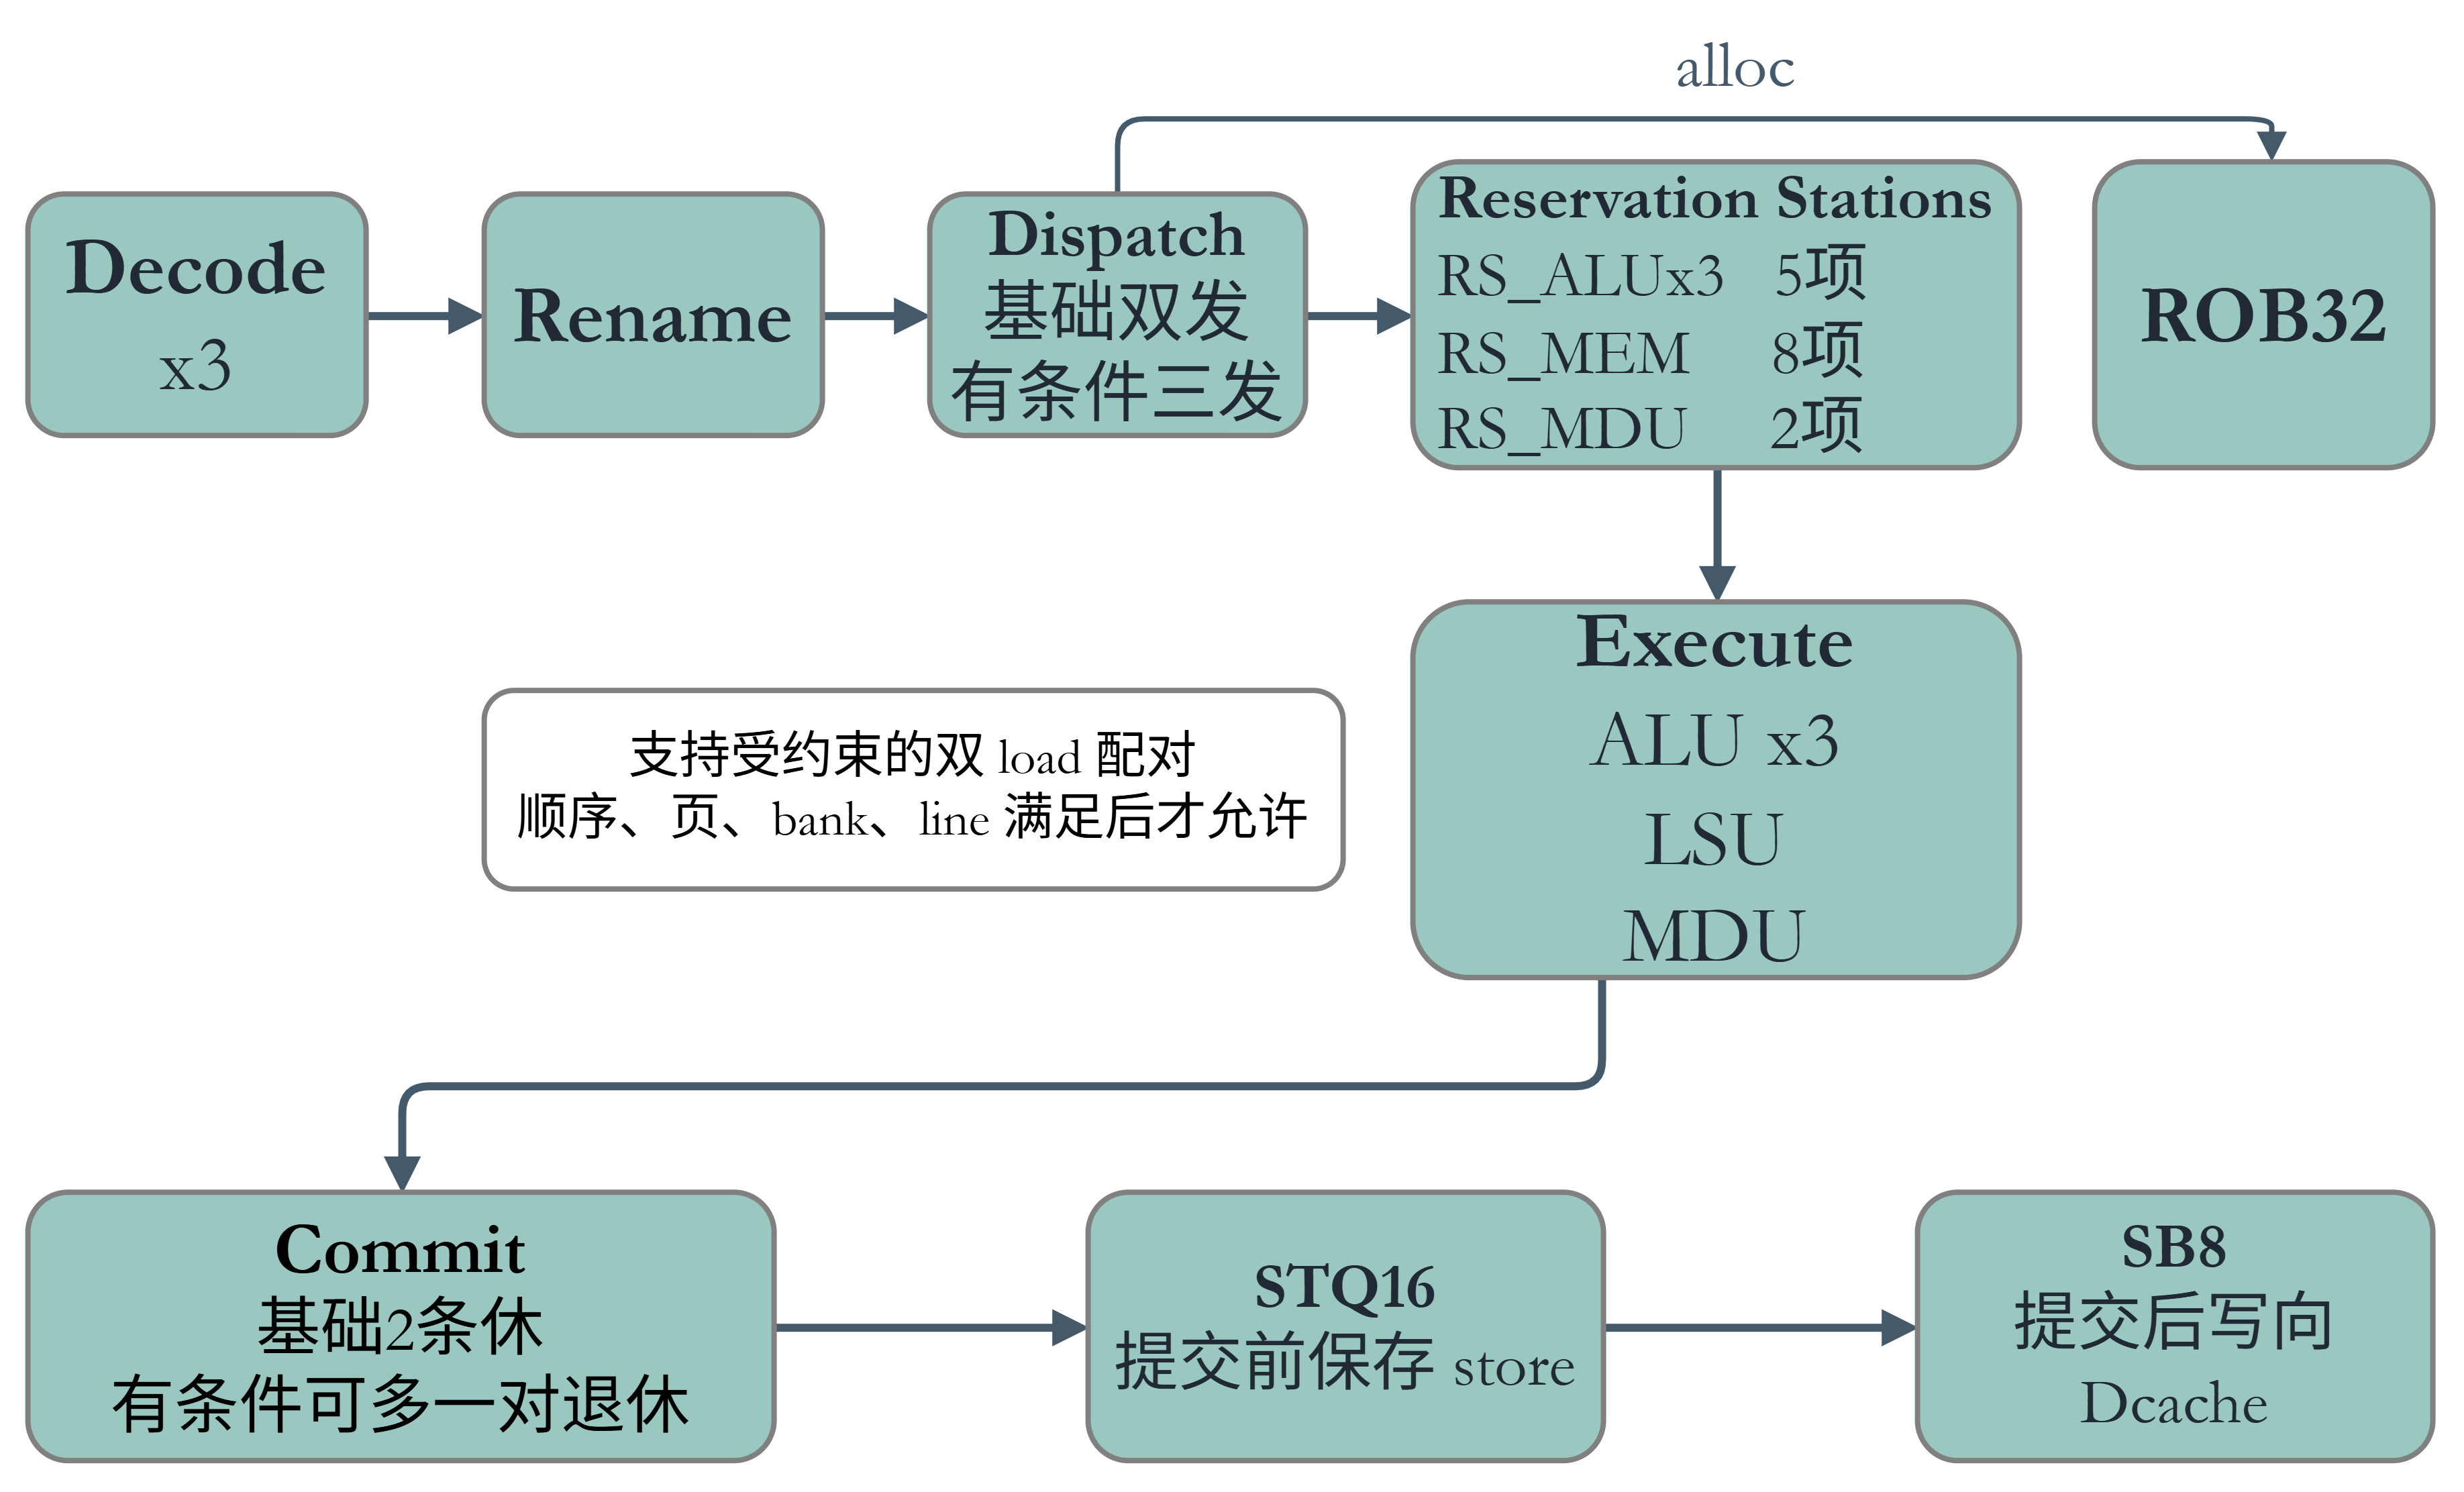
\includegraphics[width=0.95\textwidth]{figure/backend.png}
  \caption{后端架构图}
  \label{fig:backend}
\end{figure}

后端采用“2 宽基线、机会式三宽”的乱序组织，逻辑阶段为译码、重命名、分发、保留站发射、执行写回和按序提交。寄存器依赖以 ROB 编号表示，运算结果保存在 ROB；ARF 只在提交时更新，是例外或误预测恢复后的架构状态。

\subsubsection{译码与重命名}

IB 的前两条指令进入常规译码路径；第三条在资源满足时通过机会式通路继续推进。译码器生成 FU 类型、独热操作码、立即数、源/目的寄存器、访存宽度、分支类型、CSR/TLB/Cache 维护标记和例外向量。

RAT 为 32 项逻辑寄存器映射表，记录 busy 状态和最新生产者的 ROB 编号。重命名级从 RAT、ARF 和已完成 ROB 项中选择源操作数，并处理同拍指令之间的 RAW/WAW 关系。写寄存器指令更新 RAT；提交时仅在退休项仍为最新生产者时清除对应 busy。

\subsubsection{分发与保留站}

分发单元补齐可从 ROB 旁路得到的源操作数，并按类型送入异构保留站：
\begin{itemize}
  \item \textbf{RS\_ALU0/1/2}：三组、每组 5 项，从就绪项中选择指令；三条均为 ALU 类且三个执行通路可接收时可同拍三发；
  \item \textbf{RS\_MEM}：8 项。完整 SoC 模式仅允许队首访存发射，以保持 Linux 和 MMIO 顺序；性能模式可在连续且已确认 cached 的窗口内扫描最多 4 项，并启用成对 Load 优化；
  \item \textbf{RS\_MDU}：2 项 FIFO，服务乘除、CSR 读、计时器、\texttt{cpucfg} 和 TLB 维护准备操作。
\end{itemize}

unknown、TLB、uncached、MMIO 或顺序敏感访存会终止年轻访存旁路。CSR 写、TLB 修改、屏障和例外等架构副作用不在发射级生效，而在提交级串行执行。

\subsubsection{执行单元}

\begin{itemize}
  \item \textbf{ALU0/1/2}：完成整数算术、逻辑、移位、比较和分支目标计算，并将结果或分支判定写回 ROB；
  \item \textbf{LSU}：由 AGU 与 DCache 访问级组成。AGU 计算虚地址、调用 MMU 并检查对齐和页例外；后级执行 STQ/SB 前递、Cache/uncached 访问和 miss 管理；
  \item \textbf{MDU}：乘法使用寄存后的 DSP 乘积，启动后一拍完成；除法先用 CLZ 对齐，再按有效位数迭代，延迟随操作数变化。
\end{itemize}

尚未提交的 Store 保存在 16 项 STQ 中，为年轻 Load 提供顺序检查与安全前递；Store 退休后转入 8 项 Store Buffer。Store Buffer 保存已提交写操作，因此全局冲刷不会清空其内容。

\subsubsection{ROB 与提交}

ROB 共 32 项，采用奇偶双体环形组织。表项保存 PC、目的寄存器、执行结果、访存信息、预测元数据、CSR/TLB 操作和例外向量。功能单元写回后置位 complete，提交级始终从队首按程序顺序检查。

正常情况下每拍最多退休两条指令。当前两条可正常提交，且后续一对均为已完成、无例外、无分支和无串行副作用的简单指令时，可同时退休下一对，峰值为 4 条。\texttt{ll}/\texttt{sc}、CSR/TLB、屏障、\texttt{cacop}、例外和 \texttt{ertn} 会限制提交宽度。

\subsubsection{统一冲刷与精确例外}

误预测、例外、\texttt{ertn} 和需要重取的特权操作均由提交级产生全局冲刷。冲刷清空前端、RAT、ROB 和各保留站的投机状态，以已提交 ARF、CSR 与 Store Buffer 为恢复基础，再从正确 PC 重新取指。该方案没有复杂的选择性历史回滚，保证了精确例外与已提交访存不丢失。
